\section{Applications and Experiments}
\label{sec:applications}

We have used the transformation framework to inject different forms of
instrumentation into several programs, both to assess the performance
impact of sampling as well as to show that sampling can offer novel
insights into program (mis)behavior.

\subsection{Sharing the Cost of Assertions}
\label{sec:share}

In conventional usage, C \texttt{assert()} calls are used during
program development but are disabled (``\texttt{-DNDEBUG}'') when the
code ships to boost performance.  However, deployed programs fail in
unanticipated ways, and it would be helpful to retain some level of
assertion checking if the performance penalty were not excessive.

Programs produced by the \CCured instrumenting translator
\cite{POPL_'02*128} are extreme examples of assertion-dense code.
\CCured analyzes programs written in C and attempts to prove,
statically, that most pointer operations are memory safe.  Where this
cannot be done, \CCured inserts dynamic checks to enforce memory
safety at run time.  For purposes of our research, \CCured is simply a
source of highly assertion-dense code.  The individual assertions are
quite small and fast: array bounds checks, testing for null, etc.
However, in large numbers, their performance impact can be
considerable.  We wish to use random sampling to spread this cost
among many users.

We have applied sampling to several benchmarks taken from the Olden
\cite{Carlisle:1996:OPPWDDSDMM} and SPECINT95 \cite{SPEC95} benchmark
suites.  All programs run to completion and we are simply measuring
the overhead of performing the dynamic checks.

\subsubsection{Whole-Program Sampling}
\label{sec:share:whole}

\begin{table*}[tb]
  \centering
  \small
  \begin{tabular}{|l|rrr|rrr|}
    \hline
    & \multicolumn{3}{c|}{\textbf{function counts}} & \multicolumn{3}{c|}{\textbf{average for functions with sites}} \\
    \raisebox{1.5ex}[0pt]{\textbf{benchmark}} & \textbf{total} & \textbf{weightless} & \textbf{has sites} & \textbf{sites} & \textbf{threshold checks} & \textbf{threshold weight} \\
    \hline\hline
    bh & 66 & 14 & 50 & 11.8 & 3.7 & 9.4 \\
bisort & 15 & 3 & 11 & 3.5 & 1.8 & 2.3 \\
em3d & 17 & 5 & 11 & 5.3 & 2.9 & 4.6 \\
health & 18 & 2 & 15 & 5.5 & 2.7 & 3.0 \\
mst & 18 & 6 & 11 & 6.2 & 2.5 & 3.9 \\
perimeter & 11 & 4 & 6 & 6.3 & 2.7 & 1.8 \\
power & 22 & 5 & 17 & 4.9 & 2.7 & 2.7 \\
treeadd & 9 & 2 & 6 & 2.8 & 1.8 & 2.2 \\
tsp & 14 & 5 & 8 & 14.1 & 3.9 & 3.5 \\

    \hline
    compress & 23 & 4 & 18 & 6.3 & 2.6 & 3.7 \\
go & 382 & 12 & 361 & 14.7 & 5.9 & 4.7 \\
ijpeg & 316 & 27 & 272 & 18.5 & 5.0 & 7.3 \\
li & 377 & 16 & 336 & 6.2 & 3.2 & 2.9 \\

    \hline
  \end{tabular}
  \caption{Static metrics for \CCured benchmarks.  Olden benchmarks
    are listed first, followed by SPECINT95.}
  \label{tab:share:static}
\end{table*}

\autoref{tab:share:static} summarizes static aspects of the sampling
transformation when applied to the entirety of each benchmark.  For
each program, we give the total number of non-library functions and
the number of these that are weightless.  \CCured is a whole-program
analysis, so weightless function identification has the advantage of
being able to examine every function body.  We also count the number
of functions which directly contain at least one instrumentation site.
(What remains are those functions which contain no sites of their own
but which call other functions that do have sites.)

Considering just the functions which directly contain at least one
instrumentation site, \autoref{tab:share:static} also presents the
average number of sites per function, the average number of threshold
check points per function, and the average threshold weight for all
such points.  (Note that the product of the last two of these metrics
may exceed the first, as a single instrumentation site may fall under
more than one threshold check point.  This can be seen in the example
in \autoref{fig:code-layout} as well.)  The average site count gives
an impression of how assertion-dense the code is.  The average
threshold weight measures how effective our transformation has been in
amortizing the cost of countdown checks over multiple sites.
Single-site functions are not uncommon; thus, an average threshold
weight above two is encouraging because it suggests that overall
amortization rates are fairly good.

\begin{table}
  \centering
  \begin{tabular}{|l|rrrr|}
    \hline
    \rule{0pt}{2.5ex}
    \textbf{benchmark} & $\mathbf{10^{-2}}$ & $\mathbf{10^{-3}}$ & $\mathbf{10^{-4}}$ & $\mathbf{10^{-6}}$ \\
    \hline\hline
    bh & 1.06 & 1.14 & 1.15 & 1.15 \\
bisort & 1.04 & 1.06 & 1.07 & 1.06 \\
em3d & 1.15 & 1.20 & 1.21 & 1.21 \\
health & 1.00 & 1.02 & 1.02 & 1.02 \\
mst & 1.06 & 1.07 & 1.07 & 1.07 \\
perimeter & 0.96 & 0.97 & 0.97 & 0.97 \\
power & 0.97 & 1.00 & 1.00 & 1.00 \\
treeadd & 1.05 & 1.05 & 1.05 & 1.05 \\
tsp & 1.02 & 1.02 & 1.02 & 1.02 \\

    \hline
    compress & 1.32 & 1.38 & 1.39 & 1.39 \\
go & 0.83 & 0.97 & 1.00 & 1.00 \\
ijpeg & 1.24 & 1.32 & 1.34 & 1.34 \\
li & 1.07 & 1.16 & 1.16 & 1.19 \\

    \hline
  \end{tabular}
  \caption{Relative speedup of various sampling rates versus always checking}
  \label{tab:share:density}
\end{table}

\autoref{tab:share:density} shows the performance effect of various
sampling densities.  We take the running time of standard \CCured code
as the baseline.  We report the speedup ($>1$) or slowdown ($<1$)
relative to this baseline when sampling at various densities.  All
benchmarks were compiled using \texttt{gcc} 2.96 using standard
optimization (\texttt{-O2}).  Times were collected on a 550 MHz
Pentium III Linux machine with two gigabytes of RAM\@.  Reported
speedups represent the average of four runs; each run used a different
pre-generated bank of 1024 geometrically distributed random
countdowns.

Even at a fairly high sampling density of 1/100, more than two thirds
of our benchmarks run faster then they would if all checks were
performed.  Because each single check is so small and fast, this
suggests that we have been successful in amortizing our sampling
overhead.  The most dramatic speedups are seen in \texttt{ijpeg} (24\%
faster) and \texttt{compress} (32\% faster).  On the other hand, three
benchmarks do run slower, with \texttt{go} showing the largest
penalty.  In these cases, the time recovered by skipping 99/100 checks
is not enough to mask the added overhead of sampling.

As we reduce the sampling density to 1/1000, \texttt{power} reaches a
balance point of no measurable speedup or slowdown, while
\texttt{perimeter} remains a stubborn 3\% slower.  The \texttt{health}
benchmark crosses over and is now slightly faster with sampling.
Other benchmarks, which already showed speedups at 1/100, either
retain their position (\texttt{treeadd} and \texttt{tsp}) or show
additional boosts, with \texttt{compress} reaching an overall 38\%
speedup versus standard \CCured.  Further reducing the sampling
density to 1/10,000 shows little change, and by the time we reach
1/1,000,000 it is clear that we have reached a performance ceiling.
One benchmark continues to run slower than standard \CCured; two run
at the same speed; the remaining ten run 2\% - 39\% faster.

\subsubsection{Single-Function Sampling}

In an effort to better understand the sources of overhead, we have
performed additional experiments in which only a single function is
instrumented at a time.  This also approximates a more realistic
approach to managing code size.  The fully instrumented executables
from \autoref{sec:share:whole} range from 2\%-76\% larger than their
non-sampling counterparts.  When only a single function is
instrumented, code expansion is small enough to not be a concern.

A fully deployed system might use dynamic instrumentation to randomly
instrument a single selected function \textit{du jour}.  For the
present research, we build one executable for each site-containing
function as counted in \autoref{tab:share:static}.  All sites in other
functions are removed.  This, in turn, allows us to discover many more
weightless functions: any function which cannot transitively call the
one function being instrumented is weightless.  Thus, a suite of
single-function sampling executables may perform better, over all,
than a single executable with sampling in all functions.

\begin{figure}
  \centering
  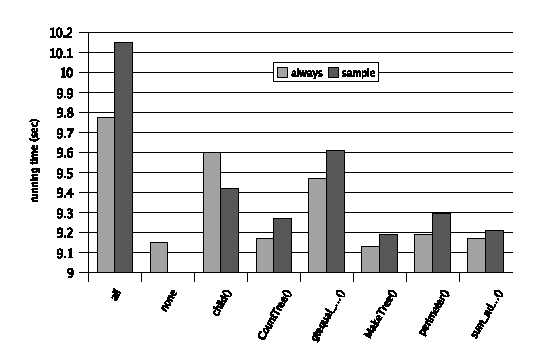
\includegraphics[width=\columnwidth]{applications/perimeter}
  \caption{\texttt{perimeter} running times with single-function
    instrumentation}
  \label{fig:share:perimeter}
\end{figure}

In the interest of space, we report only on \texttt{perimeter}: the
stubborn worst performer from the preceding experiment.  This
benchmark's small function count also makes overall results easier to
visualize.  \autoref{fig:share:perimeter} shows absolute running times
in seconds, with 1/100 sampling.  The two leftmost ``all'' bars
represent instrumenting all functions, either with checks always done
or with checks sampled.  The solo ``none'' bar represents the extreme
limit of performance: all instrumentation statically removed from all
functions.  No instrumentation scheme, with or without sampling, can
run faster than this.  The remaining bars show the running time for
each site-containing function, with that function's sites either
checked always or sampled 1/100.

Note that the vertical baseline is nine seconds, not zero, which
magnifies fairly small differences: the two leftmost bars differ by
only 4\%, the same difference reported in the ``$10^{-2}$'' column for
\texttt{perimeter} in \autoref{tab:share:density}.

Among the site-containing functions, \texttt{child()} gains a small
performance boost from sampling.  The remaining five are all
self-recursive, with between one and four recursive calls.  Our
current system treats each of these as a call to a non-weightless
function: the countdown must be exported before the call and imported
after.  A faster approach would be to transform each function to pass
the local countdown down to its recursive callees, and accept an
updated countdown back as a returned value.  Such a countdown
management strategy would be applicable any time both callee and
caller can agree on the API change; the case of self-recursive calls
is particularly straightforward.  It is worth noting that
\texttt{child()}, which does show sampling speedup, is the only
function of these six which is not self-recursive.

Benchmarks that are less dominated by recursion suggest additional
areas for improvement.  Recurring trends include:

\begin{itemize}
\item Low amortization due to lightweight regions in loops with bounds
  that are constant or fixed on entry.  A loop with iteration count
  $i$ and body weight $w$ could be treated as an acyclic region of
  weight $iw$.

\item Conservative identification of weightless functions.  Calls
  through function pointers or to externally-defined code are assumed
  to potentially recurse back to the caller.  Points-to analyses can
  improve the former; a statically checkable \texttt{weightless}
  annotation on function prototypes would resolve the later.
\end{itemize}

When multiple functions are being instrumented, we find another area
for improvement.  Some callees may not be weightless, but can never
cross more than some finite number of sites per call.  The caller of a
finite-weight function can exploit this upper limit, effectively
treating the callee as a cluster of sites of appropriate weight.

We expect that these and other optimizations will continue to improve
the performance benefit from sampling, both for single-function as
well as whole-program instrumentation.

\subsection{Bug Hunting Using Feature Elimination}

\aside{Story to tell here:
  
  Preceding experiment is all well and good if possible failure points
  are explicitly marked with assertions, but you can't expect that in
  general.  Instead, we want to make fairly wild guesses about
  possible problems, then eliminate these in light of their behavior
  in actual runs.  Function return values are a good place to make
  these guesses, as they are often used to indicate success or failure
  of a given operation.  Experiment with \texttt{ccrypt} shows that we
  can reliably rediscover a known fatal error by sampling and
  filtering function return values.
  
  We didn't have the \texttt{ccrypt} experiment when we first wrote up
  the \texttt{bc} experiment, so \autoref{sec:debug} already spends
  some time introducing the idea of counter triples, randomized input
  to simulate a large user community, etc.  Some of that text should
  probably be lifted up and placed here instead.}

\subsection{Statistical Debugging}
\label{sec:debug}

Sampled information about program behavior can be thought of as a
database.  Data mining techniques, then, may reveal important
information about the aggregate behavior of many runs.  Of particular
interest to us is finding and fixing bugs.  We now illustrate how
mining of sampled program behavior can help direct software engineers
to the root cause of difficult bugs.

Because we do not have ready access to thousands of users, we simulate
a large user community by using randomly generated inputs in the
spirit of the Fuzz project~\cite{MKLMMNS95}.  Our selected target is
version 1.06 of the GNU implementation of \texttt{bc}.  We find that
feeding \texttt{bc} nine megabytes of random input causes it to crash
roughly one time in four.  \disregard{While this would be an unusually
  high failure rate for shipping software under normal usage patterns,
  we expect that users experiencing crashes will be more likely to
  opt-in to a trace reporting system.  Thus, this may be a reasonable
  ratio to expect if most crashes and a few non-crashes are reported.}

Quick perusal of the stack trace at a typical failure is discouraging.
The crash occurs several frames deep inside the C library's
\texttt{malloc()} function: a sure sign of heap corruption.  Such bugs
are especially pernicious because the actual corruption may have
happened well before the ultimate crash \cite{Eisenstadt1993b}.

We instrument \texttt{bc} to guess and randomly check a large number
of possible invariants.  Our goal is to identify predicates that hold
when the program succeeds, but which are violated when the program
crashes.  We cast an extremely broad net, but with an eye toward
pointer use errors and buffer overruns.  For pointer use, null
pointers are clearly of interest.  Relative addresses of pointers may
be interesting as well, as this may capture cases where one pointer
scans within a second pointed-to buffer.  Checking pointer/pointer
equality may reveal aliasing which, when not anticipated by the
programmer, can lead to dangling ``wild'' pointer bugs.  Scalar
variables serve as array indexes, pointer offsets, and in many other
roles; relationships among scalars may reveal buffer overruns,
unanticipated consequences of negative values, invalid enumeration
constants, or a variety of other problems.

At any direct assignment to a scalar variable \texttt{a}, we identify
all other local or global variables $\{ \mathtt{b}_1, \mathtt{b}_2,
\dots, \mathtt{b}_n \}$ which are also in scope and which have the
same type.  We then compare the updated \texttt{a} to each
$\mathtt{b}_i$, and note whether \texttt{a} was less than, equal to,
or greater than $\mathtt{b}_i$.  Even with very sparse sampling, a
direct trace of these comparisons would overwhelm both client,
network, and server.  Instead, we locally reduce the trace by merely
counting how often each of the three relative orderings appeared.  We
compare pointers to same-typed pointers as well, and additionally
compare each pointer for equality with null.  One comparison between
\texttt{a} and $\mathtt{b}_i$, which bumps one of three counters, is
considered to be one instrumentation site subject to random sampling.
When an instrumented application terminates, it emits the vector of
counter triples along with a flag indicating whether it completed
successfully or was aborted by a fatal signal.

As expected, this gives us a large number of candidate predicates:
10,050 counter triples, or 30,150 counters in all.  Because our
guesses are so crude, the vast majority of these are of no interest:
either they compare completely unrelated variables, or they express
relationships which behave identically in both successful and failed
runs.  The challenge is to find those few candidate predicates which
truly matter.

\subsubsection{Crash Prediction Using Logistic Regression}

To find these few important predicates, we recast the bug hunt as a
statistical analysis problem.  Each run of \texttt{bc} constitutes one
sample point consisting of 30,150 observed \termdef{features} and one
binary \termdef{outcome} ($0 = \text{succeeded}, 1 = \text{crashed}$).
In C, a misbehaving program can sometimes ``get lucky'': it may
violate memory safety yet not crash.  Hence the outcome label is
non-deterministic.  Given numerous data points (sampled runs), we
would like to identify a narrow subset of our 30,150 features which
are relevant to predicting the succeeded/crashed outcome.  This is
equivalent to the machine learning problem of learning a binary
classifier with feature selection, i.e.\ using as few input features
as possible.

In the classification setting, we take a set of data with known binary
output (a training set), and attempt to learn a binary classifier that
gives good predictions on a test set.  The learning process usually
involves additional parameters whose values can be determined using a
validation set.  In our case, the end goal is to narrow down the set
of features.  Hence our method will have to balance good
classification performance with aggressive feature selection.

A binary classifier takes feature values as inputs, and outputs a
prediction of either $0$ or $1$.  \termdef{Logistic regression}
\cite{Hastie01} is a method of learning a binary classifier where the
output function is assumed to be logistic.  The logistic function is a
continuous ``S''-shaped curve approaching 0 on one end, and 1 on the
other.  The output can be interpreted as a probability measure of how
likely the data point falls within class 0 or 1.  Quantizing the
logistic function output then gives us a binary classifier: if the
output is greater than $1/2$, then the data point is classified as
class 1 (a crash), otherwise it falls under class 0 (a successful
run).  Feature selection can be achieved by \termdef{regularizing} the
function parameters to ignore most input features.

\aside{Alice writes: this paragraph should be revisited after we
  finish the experimental results.}
  
While other ways of combined classification and feature selection
exist, none of them are particularly well-suited for this problem.
Some methods \cite{Golub:MCC:1999,Tibshirani2002} calculate a
univariate correlation coefficient independently for each feature;
other methods, such as decision trees \cite{00000048}, are more
computationally intensive.  In our dataset, the features are clearly
not independent of each other, and the size of the problem can
potentially be too large for more computationally intensive methods.
Furthermore, logistic regression is a discriminative classification
method, and thus does not make any assumptions about the underlying
distribution of the input.  This is crucial since our features arise
from a decidedly artificial process and would be difficult to
characterize using simple distributions.

Suppose our training set $\mathcal{D}$ consists of $M$ data points
$(x_1,y_1), \ldots, (x_M, y_M) $, where each $x_i \in \Real^N$ denotes
a vector of input predicate counters, and each $y_i = \{0, 1\}$
denotes the corresponding output label.  To learn a good classifier,
we can maximize the \termdef{log likelihood} of the training set.
%%
\begin{equation*}
  \begin{split}
    LL(\mathcal{D}) \:=\:
    \sum_{i=1}^M \, [ & y_i \log P(Y = 1 | x) \\
    + & (1 - y_i) \log (1 - P(Y = 1 | x)) ]
  \end{split}
\end{equation*}
%%
Here the output labels $y_i$ are used as indicator functions to zero
out exactly one of the two terms in each summand.  In logistic
regression, the distribution $P(Y=1|x)$ is modeled as the logistic
function $\mu_{\tilde{\beta}}(x)$ with parameters $\tilde{\beta} = \langle \beta_0 \in
\Real, \beta \in \Real^N \rangle$.
%%
\begin{equation*}
  P(Y = 1 | x) = \mu_{\tilde{\beta}} (x) = \frac{1}{1 + \exp(- \beta_0 - \beta^T x)}
\end{equation*}
%%
The logistic parameters $\beta_0$ and $\beta$ take on the respective roles as
the intercept and slope of the classifier, and essentially weigh the
relative importance of each feature in the final outcome.  We expect
most of the input features to have no influence over the success or
failure of the program, so we place an additional constraint that
forces most of the $\tilde{\beta}$'s toward zero.  This is accomplished by
subtracting a penalty term based on the L1-norm $\norm{\tilde{\beta}}_1 =
\sum_{j=0}^M \abs{\beta_j}$.  We can tune the importance of this
\termdef{regularization term} through a \termdef{regularization
  parameter} $\lambda$.  The penalized log likelihood function is:
%%
\begin{equation*}
  \begin{split}
    LL (\tilde{\beta} | \mathcal{D}, \lambda ) \:=\:
    & \sum_{i=1}^M \, [y_i \log \mu_{\tilde{\beta}} (x_i) + (1 - y_i) \log (1 - \mu_{\tilde{\beta}} (x_i))] \\
    & - \lambda \norm{\beta}_1
  \end{split}
\end{equation*}

\subsubsection{Bug Hunting in \texttt{bc}}

Our \texttt{bc} dataset consists of 4390 runs with distinct random
inputs and distinct randomized $1/1000$ sampling, of which 2729 are
randomly chosen for training, 322 for validation, and 1339 for
testing.  Although there are 30,150 raw features, many can be
discarded immediately: in the training set 27,242 features are always
zero.  Hence the effective number of features used in training is
2908.  (Beyond simplifying the statistical analysis, this degree of
regularity means that counter reports are highly compressible: good
news for deployed users with small hard drives or slow modems.)
Furthermore, to make the magnitude of the $\beta$ parameters comparable,
the feature values have to be on the same scale.  Hence all the input
features are shifted and scaled to lie between $[0,1]$, then
normalized to have unit sample variance.  A suitable value for the
regularization parameter $\lambda$ is determined through validation to be
$0.3$.  The model is then trained using stochastic gradient ascent to
reach a local maximum of the penalized log likelihood.  Using a
learning rate of $10^{-5}$, the model usually converges within sixty
iterations through the training set.  This takes roughly thirty
minutes in MATLAB on a 1.8 GHz Pentium 4 CPU with 1 GB of RAM.

Once the model has been trained, predicates with the largest $\beta$
coefficients suggest where to begin looking for the bug.  In our case,
the top five ranked coefficients are well-separated in magnitude from
the rest, and show an unmistakable trend:

\newcounter{feature}
\begin{list}{\arabic{feature}.}{\usecounter{feature}\setlength{\itemsep}{0pt}\setlength{\parsep}{0in}\ttfamily\small}
\item storage.c:176: more\_arrays(): indx > scale
\item storage.c:176: more\_arrays(): indx > use\_math
\item storage.c:176: more\_arrays(): indx > opterr
\item storage.c:176: more\_arrays(): indx > next\_func
\item storage.c:176: more\_arrays(): indx > i\_base
\end{list}

\begin{figure}
  \centering
  \small
  \listinginput{152}{applications/more_arrays.c}
  \caption{Suspect \texttt{bc} function \texttt{more\_arrays()}.  All
  top-ranked crash-predicting features point to large values of
  \texttt{indx} on line 176.}
  \label{fig:bc:more-arrays}
\end{figure}

The source code for \texttt{more\_arrays()} appears in
\autoref{fig:bc:more-arrays}.  An comment earlier in the same file
suggests that this one of a suite of ``three functions for increasing
the number of functions, variables, or arrays that are needed''.  The
logic is a fairly clear instance of the buffer reallocation idiom,
even to one unfamiliar with the code: line 167 allocates a larger
chunk of memory; line 171 is the top of a loop that transfers values
over from the old, smaller array; line 176 completes the resize by
zeroing out the new extra space.  As the comment suggests, there are
two similar functions (\texttt{more\_functions()} and
\texttt{more\_variables()}) nearby that do largely the same thing with
different storage pools.  The text of these three functions is nearly
identical, but each uses different global variables (e.g.
\texttt{a\_count} versus \texttt{f\_count} versus \texttt{v\_count}).

The top ranked predicates seem bizarre at first glance, because the
variables they relate do not appear to have any real connection to
each other or to \texttt{more\_arrays()}.  For example, \texttt{scale}
tracks significant digits for floating point calculations, while
\texttt{use\_math} records whether an initial math library is to be
loaded.  Why would crashes tend to happen when local variable
\texttt{indx} exceeds these seemingly unrelated globals on this
particular line?  An obvious hypothesis is that \texttt{indx} is
simply unusually large in such cases.  If \texttt{indx} is large, then
it will tend to be larger than any number of otherwise unrelated
variables.  Perhaps crashes occur when the input to \texttt{bc}
defines unusually large numbers of arrays.

Closer scrutiny of \texttt{more\_arrays()} quickly reveals this to be
the case.  The allocation on line 167 requests space for
\texttt{a\_count} items.  The copying loop on line 171 ranges from
\texttt{1} through \texttt{old\_count - 1}.  The zeroing loop on line
176 continues on from \texttt{old\_count} through \texttt{v\_count -
  1}.  And here we find the bug: the new storage buffer has room for
\texttt{a\_count} elements, but the second loop is incorrectly bound
by \texttt{v\_count} instead.  After a quick glimpse at the
neighboring \texttt{more\_variables()} function it is clear that
\texttt{more\_arrays()} was created by copying and pasting
\texttt{more\_variables()} and then changing names like
\texttt{v\_count} and \texttt{v\_names} to \texttt{a\_count} and
\texttt{a\_names}.  The loop bound on line 176 was missed in the
renaming.

The logistic regression model points us at the buggy line, the buggy
variable, and even reveals something of the conditions under which the
bug will appear.  Having found the bug, it is reasonable to ask
whether the statistical analysis could have pointed at it even more
directly.  The mistaken use of \texttt{v\_count} instead of
\texttt{a\_count} on line 176 means that a buffer overrun occurs when
\texttt{indx > a\_count} on line 176.  This does correspond to a
predicate sampled by our system, but this predicate is ranked 240th in
the trained model.  Why was this, the smoking gun, not ranked first?

There are several reasons to consider.  Samples are taken randomly,
while the model itself is trained using stochastic gradient ascent.
Thus, a degree of noise is fundamental to the process.  Even crashing
is not guaranteed: out of 320 runs in which sampling spotted
\texttt{indx > a\_count} at least once, 66 did not crash.  Thus, C
programs can ``get lucky'', meaning that this is not a strict
$\text{overrun} \implies \text{crash}$ implication.  Manual inspection
of the data reveals a high degree of redundancy among many
instrumentation sites within \texttt{more\_arrays()}, meaning that the
model has several features to choose from which have equivalent
predictive power.  This may suggest that our counters are too
fine-grained; that we are distinguishing many behaviors which are in
fact so tightly interrelated as to be equivalent.  Improving our
instrumentation scheme and fine-tuning the statistical analysis
methodology are key areas for continued development.

\aside{Add some treatment of the fact that our model predicts crashes
  \texttt{better} than an artificial model built using only the
  smoking gun.  Even taking the single top-ranked feature in isolation
  gives a model that outperforms the smoking gun.  This is certainly
  interesting, and worth reporting, but I'm not sure what to say about
  it by way of explaining \texttt{why} this happens.}

\aside{Need to add discussion of overhead: compare no instrumentation,
  sampled instrumentation, and unconditional instrumentation.} 

This bug seems clear enough once found.  However it has been present
and undiscovered at least since 1992 (the time\-stamp on this file in
the oldest version of GNU \texttt{bc} that we can find).  Many bugs
are obvious only once one knows where to look.  The logistic
regression results directed us to one misbehaving variable on one line
of code, out of 8910 lines in \texttt{bc} as a whole.  Our approach
does not automatically find and fix bugs.  But it does suggest where
to start looking, and what sort of scenarios (large \texttt{indx}) to
consider.  Although we are still learning about the capabilities of
this system, and how to interpret its results, we believe that
statistically guided debugging has the potential to make the process
of finding and fixing bugs more efficient.
